\documentclass[twocolumn,10pt]{article}

\usepackage[margin=0.72in, columnsep=0.26in]{geometry}
\usepackage[utf8]{inputenc}
\usepackage[T1]{fontenc}
\usepackage{lmodern}
\usepackage{microtype}
\usepackage{amsmath,amssymb}
\usepackage{graphicx}
\usepackage{booktabs}
\usepackage{array}
\usepackage{multirow}
\usepackage[numbers,sort&compress]{natbib}
\usepackage{xcolor}
\usepackage{caption}
\usepackage{stfloats}
\usepackage{hyperref}

\definecolor{navy}{RGB}{18,52,96}
\definecolor{slate}{RGB}{70,85,105}
\hypersetup{
  colorlinks=true,
  linkcolor=navy,
  citecolor=navy,
  urlcolor=navy,
  pdftitle={Autonomous Multiphysics Co-Design of Rare-Earth-Free Traction Motors Coupled to SiC Inverter kVA, Centrifugal Elasticity, and Cold-Soak Demagnetization},
  pdfauthor={Jack Jay}
}

\captionsetup{font=small, labelfont=bf}
\setlength{\parskip}{3pt}

\title{\vspace{-1.4em}\Large\bfseries Autonomous Multiphysics Co-Design of Rare-Earth-Free Traction Motors Coupled to SiC Inverter kVA, Centrifugal Elasticity, and Cold-Soak Demagnetization}

\author{
  \normalsize\textbf{Jack Jay}\\[2pt]
  \small\color{slate} Independent Researcher (\href{https://jackjay.io}{jackjay.io}) --- Assisted by Autonomous Multi-Agent Physics Verification Pipeline\\[-2pt]
  \small\color{slate} Open-Source Code, CAD Specs \& FEA Ledgers: \href{https://github.com/theguysaccount/open-physics-autoresearch}{github.com/theguysaccount/open-physics-autoresearch}
}
\date{\small Preprint Manuscript --- Version 1.0 (November 2026)}

\begin{document}
\twocolumn[
  \begin{@twocolumnfalse}
    \maketitle
    \vspace{-1.0em}
    \begin{abstract}
      \noindent Electric vehicle and industrial traction drives remain heavily dependent on dysprosium-doped sintered NdFeB magnets ($\approx\$115/\text{kg}$) because conventional rare-earth-free designs fail under three coupled real-world multiphysics constraints frequently omitted from idealized studies: (1) low power factor ($\cos\phi$) inflating 400~V SiC traction inverter apparent-power rating (kVA) and total drive cost, (2) 2D centrifugal overspeed fracture on thin rotor flux-barrier bridges at $1.2\,\omega_{\max}=14{,}400\;\text{rpm}$, and (3) cold-soak ($-30\,^\circ\text{C}$) irreversible demagnetization of ceramic ferrite under peak launch current. We apply a locked four-stage autonomous scientific discovery pipeline---executing $1{,}296$ exact nonlinear 2D Maxwell finite-element (\texttt{Gmsh} + \texttt{Numba} Newton--Raphson with exact node-matching sliding-band rotation) and 2D plane-stress centrifugal elasticity evaluations across 16 CPU cores---inside a fixed $4.40\;\text{L}$ traction envelope ($200\;\text{mm}$ OD $\times 140\;\text{mm}$ stack, $400\;\text{V}$ DC bus, $0.5\;\text{mm}$ cut-edge degraded lamination zone, AC proximity copper loss, and 3D analytical end-winding $R_{\text{ph}}/L_{\text{ew}}$). Across three head-to-head evolutionary tracks independently verified on a $2\times$ refined mesh ($n_{\text{steps}}=24$):
      \begin{enumerate}\setlength{\itemsep}{1pt}\setlength{\topsep}{2pt}
        \item \textbf{Zero-Magnet Pure SynRM (\texttt{T2}, \texttt{4p/48s 4B}, $352$ evals) Hits an Unbreakable System-Cost Wall:} Even with unconstrained asymmetric 4-barrier evolution and $\text{SF}=1.52$ overspeed compliance, pure reluctance stalls at $162.1\;\text{Nm}$ peak launch torque (below the $185\;\text{Nm}$ EV target) and $\cos\phi=0.652$, bloating the required 400~V SiC inverter to $178.5\;\text{kVA}$ ($\$1{,}513$) and pushing total drive cost to $\$1{,}747$---$55\%$ costlier than optimized NdFeB despite $\$0$ magnets.
        \item \textbf{Rare-Earth-Free Ceramic Ferrite Co-Design (\texttt{T3}, \texttt{6p/54s 2B} Thick Asymmetric Double-V, $640$ evals) Beats Commercial 8-Pole NdFeB and Reaches $2.2\%$ Cost Parity with Autoresearch-Optimized Dy-NdFeB:} Autoresearch abandoned saliency-starved \texttt{8p/48s} and thin-barrier \texttt{4p} templates, converging onto a 6-pole 54-slot ($q=3$) stator with an enlarged $137.05\;\text{mm}$ rotor OD ($+15.1\;\text{mm}$ over NdFeB) and two ultra-thick ($7.44\;\text{mm}$ / $5.84\;\text{mm}$) asymmetric flux-concentrating \texttt{FB12B} La--Co ceramic ferrite barriers ($2.23\;\text{kg}$, $\$12$ magnet BOM) braced by $2.90\;\text{mm}$ / $1.81\;\text{mm}$ central structural steel posts. Verified at $2\times$ fine mesh and $24$ rotation steps, \texttt{T3} delivers $93.10\%$ WLTC drive-system efficiency (motor + SiC inverter), $\cos\phi=0.809$, $99.8\;\text{kVA}$ inverter rating (smaller than commercial \texttt{8p/48s} NdFeB's $105.5\;\text{kVA}$), $9.46\%$ WLTC torque ripple ($6.3\%$ at rated \texttt{OP2}---asymmetric barrier wing angles alone cutting ripple by $51.5\%$), $\text{SF}=1.52$ at $14{,}400\;\text{rpm}$, $+0.019\;\text{T}$ cold-soak ($-30\,^\circ\text{C}$) demagnetization margin, and $\$1{,}153$ total drive cost ($-\$210$ / $-15.4\%$ below commercial \texttt{8p} NdFeB $\$1{,}363$, and within $\$25$ / $+2.2\%$ of autoresearch-optimized \texttt{6p/54s} Dy-NdFeB $\$1{,}128$).
      \end{enumerate}
      \vspace{0.5em}
      \noindent\textbf{Keywords:} Rare-earth-free electric motors; Ferrite PM-assisted synchronous reluctance; Nonlinear 2D Maxwell FEA; SiC inverter kVA co-design; Asymmetric flux barriers; Centrifugal elasticity; Cold-soak demagnetization; Autonomous optimization.
    \end{abstract}
    \vspace{0.7em}
  \end{@twocolumnfalse}
]

\section{Introduction and Multiphysics Motivation}

Permanent-magnet synchronous traction motors dominate electric vehicles because sintered dysprosium-doped NdFeB delivers high torque density and near-unity power factor \citep{pellegrino2012comparison,cai2016asymmetric}. Yet heavy rare-earth supply concentration and volatile alloy pricing ($\approx\$115/\text{kg}$ for \texttt{N42SH}) create acute strategic and cost risk. Decades of foundational work on synchronous reluctance (\texttt{SynRM}) \citep{vagati1994synchronous,boldea1996reluctance} and ceramic ferrite PM-assisted synchronous reluctance (\texttt{PMa-SynRM}) \citep{bianchi2009torque,sanada2014ferrite} demonstrated that reluctance torque can replace most rare-earth magnet torque, yet mass-market EV adoption remains limited by three tightly coupled failure modes:
\begin{enumerate}\setlength{\itemsep}{1pt}
  \item \textbf{SiC Inverter-kVA Blowup ($\cos\phi$ Coupling):} Eliminating magnets without boosting power factor forces the 400~V SiC traction inverter to supply $1/\cos\phi$ higher peak current, often adding $\$300\text{--}\$600$ in SiC silicon that erases the magnet savings.
  \item \textbf{Centrifugal Overspeed Fracture vs.\ Leakage Flux:} High saliency demands ultra-thin rotor bridges and minimal structural ribs, which fracture under $1.2\,\omega_{\max}=14{,}400\;\text{rpm}$ centrifugal loads when realistic non-bonded magnet masses are modeled.
  \item \textbf{Opposite Thermal Demagnetization Physics:} Unlike NdFeB (whose coercivity drops at hot $+140\,^\circ\text{C}$), strontium/La--Co ceramic ferrite (\texttt{TDK FB12B}) exhibits a \emph{positive} coercivity temperature coefficient---its worst-case irreversible demagnetization occurs at \emph{cold soak} ($-30\,^\circ\text{C}$, $B_{\text{knee}}=+0.10\;\text{T}$), while its lowest torque flux occurs at hot ($+140\,^\circ\text{C}$, $B_r=0.353\;\text{T}$).
\end{enumerate}

Here we embed every one of these constraints---plus $0.5\;\text{mm}$ mechanical cut-edge lamination degradation \citep{bali2017cutedge}, Bertotti harmonic iron loss \citep{bertotti1988general}, slot-leakage AC proximity copper loss, and 3D end-winding resistance and leakage inductance \citep{pyrhonen2014design}---inside a fast, exact nonlinear 2D FEA harness and deploy a 16-core four-layer evolutionary search over discrete pole-slot topology, active magnet layout, unconstrained asymmetric rotor/stator geometry, and harmonic current injection.

\section{Locked Multiphysics FEA Harness and Governing Equations}

\subsection{Nonlinear 2D Magnetostatics \& Sliding-Band Rotation}
A 1-pole anti-periodic sector ($\theta\in[0,\pi/p]$, $A_z(r,\theta+\pi/p)=-A_z(r,\theta)$) is meshed cleanly via \texttt{Gmsh} OpenCASCADE \citep{geuzaine2009gmsh} across five integer-slot topologies: \texttt{8p/48s}, \texttt{6p/36s}, \texttt{6p/54s}, \texttt{4p/36s}, and \texttt{4p/48s}. The magnetic vector potential $A_z$ satisfies the nonlinear weak form:
\begin{equation}
  \int_\Omega \nu(B^2)\,\nabla v\cdot\nabla A_z\,d\Omega
  = \int_\Omega J_z v\,d\Omega + \int_{\Omega_{\text{m}}} \nu_m\!\left(B_{r,x}\frac{\partial v}{\partial y} - B_{r,y}\frac{\partial v}{\partial x}\right) d\Omega,
  \label{eq:maxwell}
\end{equation}
solved via exact analytical-Jacobian damped Newton--Raphson to $10^{-6}$ residual using a strictly monotone PCHIP $\nu(B^2)$ spline calibrated to \texttt{M270-35A} ($0.35\;\text{mm}$) electrical steel. Every steel element whose centroid lies within $d_{\text{cut}}=0.5\;\text{mm}$ of an air, slot, or barrier boundary is automatically tagged with cut-edge degraded permeability ($+58\%$ knee $H$) and $1.75\times$ hysteresis loss \citep{bali2017cutedge}.

Two analytically generated structured uniform triangular rings spanning $[r_{g1}, r_{g3}]=[r_{\text{ro}}+0.25g,\, r_{\text{ro}}+0.75g]$ with $N_\theta=72$ uniform segments per pole enable exact node-for-node sliding-band rotation without remeshing and zero-noise Arkkio torque integration \citep{arkkio1987analysis}:
\begin{equation}
  T_{\text{Arkkio}} = \frac{2p\,L_{\text{stk}}}{\mu_0\,(r_{g3}-r_{g1})} \iint_{\text{1-pole }[r_{g1},r_{g3}]} r\,B_r B_\theta\,dA.
  \label{eq:arkkio}
\end{equation}

\subsection{2D Plane-Stress Centrifugal Elasticity FEA}
On the identical rotor triangulation (with rotational periodicity $\mathbf{u}(\theta_p)=\mathbf{R}(\theta_p)\mathbf{u}(0)$ and clamped shaft bore $r=R_{\text{sh}}=26\;\text{mm}$), 2D plane-stress elasticity is solved at $14{,}400\;\text{rpm}$ ($1.2\,\omega_{\max}$) under centrifugal body force $\mathbf{f}_c = \rho_e \omega^2 \mathbf{r}$. Magnets are modeled conservatively as compliant load-transferring bodies ($E=1.5\;\text{GPa}$, full density $\rho_{\text{fer}}=4900$, $\rho_{\text{Nd}}=7500\;\text{kg/m}^3$) with $15\;\text{MPa}$ clearance potting ($0.007\%$ of steel $E=205\;\text{GPa}$) so steel ribs and bridges carry $>99.9\%$ of all centrifugal loads. Hard safety gates enforce $t_{\text{bridge}}\ge 0.80\;\text{mm}$, $t_{\text{rib}}\in\{0\}\cup[\ge 0.80\;\text{mm}]$, and area-smoothed nodal von Mises safety factor $\text{SF}=\sigma_y/\sigma_{\text{vM}}\ge 1.50$ ($\sigma_y=420\;\text{MPa}$).

\subsection{Losses, WLTC Drive Cycle, and SiC Inverter-kVA Cost}
Locked envelope: $D_{\text{so}}=200\;\text{mm}$, $L_{\text{stk}}=140\;\text{mm}$ ($4.40\;\text{L}$), $V_{\text{dc}}=400\;\text{V}$ ($V_{\text{ph,pk}}\le 219.4\;\text{V}$), $k_{\text{fill}}=0.45$, $g\ge 0.65\;\text{mm}$. Four WLTC operating points (\texttt{OP1}: $2000\;\text{rpm}/40\;\text{Nm}$, $w=0.30$; \texttt{OP2}: $4000/75$, $0.30$; \texttt{OP3}: $7500/45$, $0.25$; \texttt{OP4}: $11500/30$, $0.15$; $J_{\text{cont}}\le 12.5\;\text{A/mm}^2$) plus peak launch \texttt{OP5} ($2500\;\text{rpm}$, $T_{\text{peak}}\ge 185\;\text{Nm}\times 0.97$, $J_{\text{peak}}\le 24\;\text{A/mm}^2$) are evaluated via multi-step nonlinear FEA at hot $+140\,^\circ\text{C}$ magnet remanence. Total losses sum DC copper ($120\,^\circ\text{C}$ incl.\ 3D end-winding $l_{\text{ew}}=1.55\tau_p+25\;\text{mm}$), slot-leakage AC proximity copper ($\propto B_{\text{slot}}^2\omega_e^2$), Bertotti stator+rotor harmonic iron loss \citep{bertotti1988general} (with $1.75\times$ cut-edge hysteresis), bearing/windage drag, and 12~kHz SiC MOSFET conduction+switching loss. Total drive system cost couples motor active BOM ($1.35\times$ stamped \texttt{M270-35A} at $\$2.40/\text{kg}$, Cu $\$10.50/\text{kg}$, \texttt{FB12B} $\$5.50/\text{kg}$, \texttt{N42SH} $\$115/\text{kg}$, $+\$95$ fixed) with 400~V SiC inverter hardware:
\begin{equation}
  \text{Cost}_{\text{inv}} = \$180 + \$7.50\cdot S_{\text{inv,kVA}}, \qquad
  S_{\text{inv,kVA}} = \frac{1.5\,V_{\text{ph,max}}\,I_{\text{inv,pk}}}{1000}.
  \label{eq:inv_cost}
\end{equation}

\section{Results: 1,296-Eval Autoresearch & Phase Boundary}

\begin{figure*}[t]
  \centering
  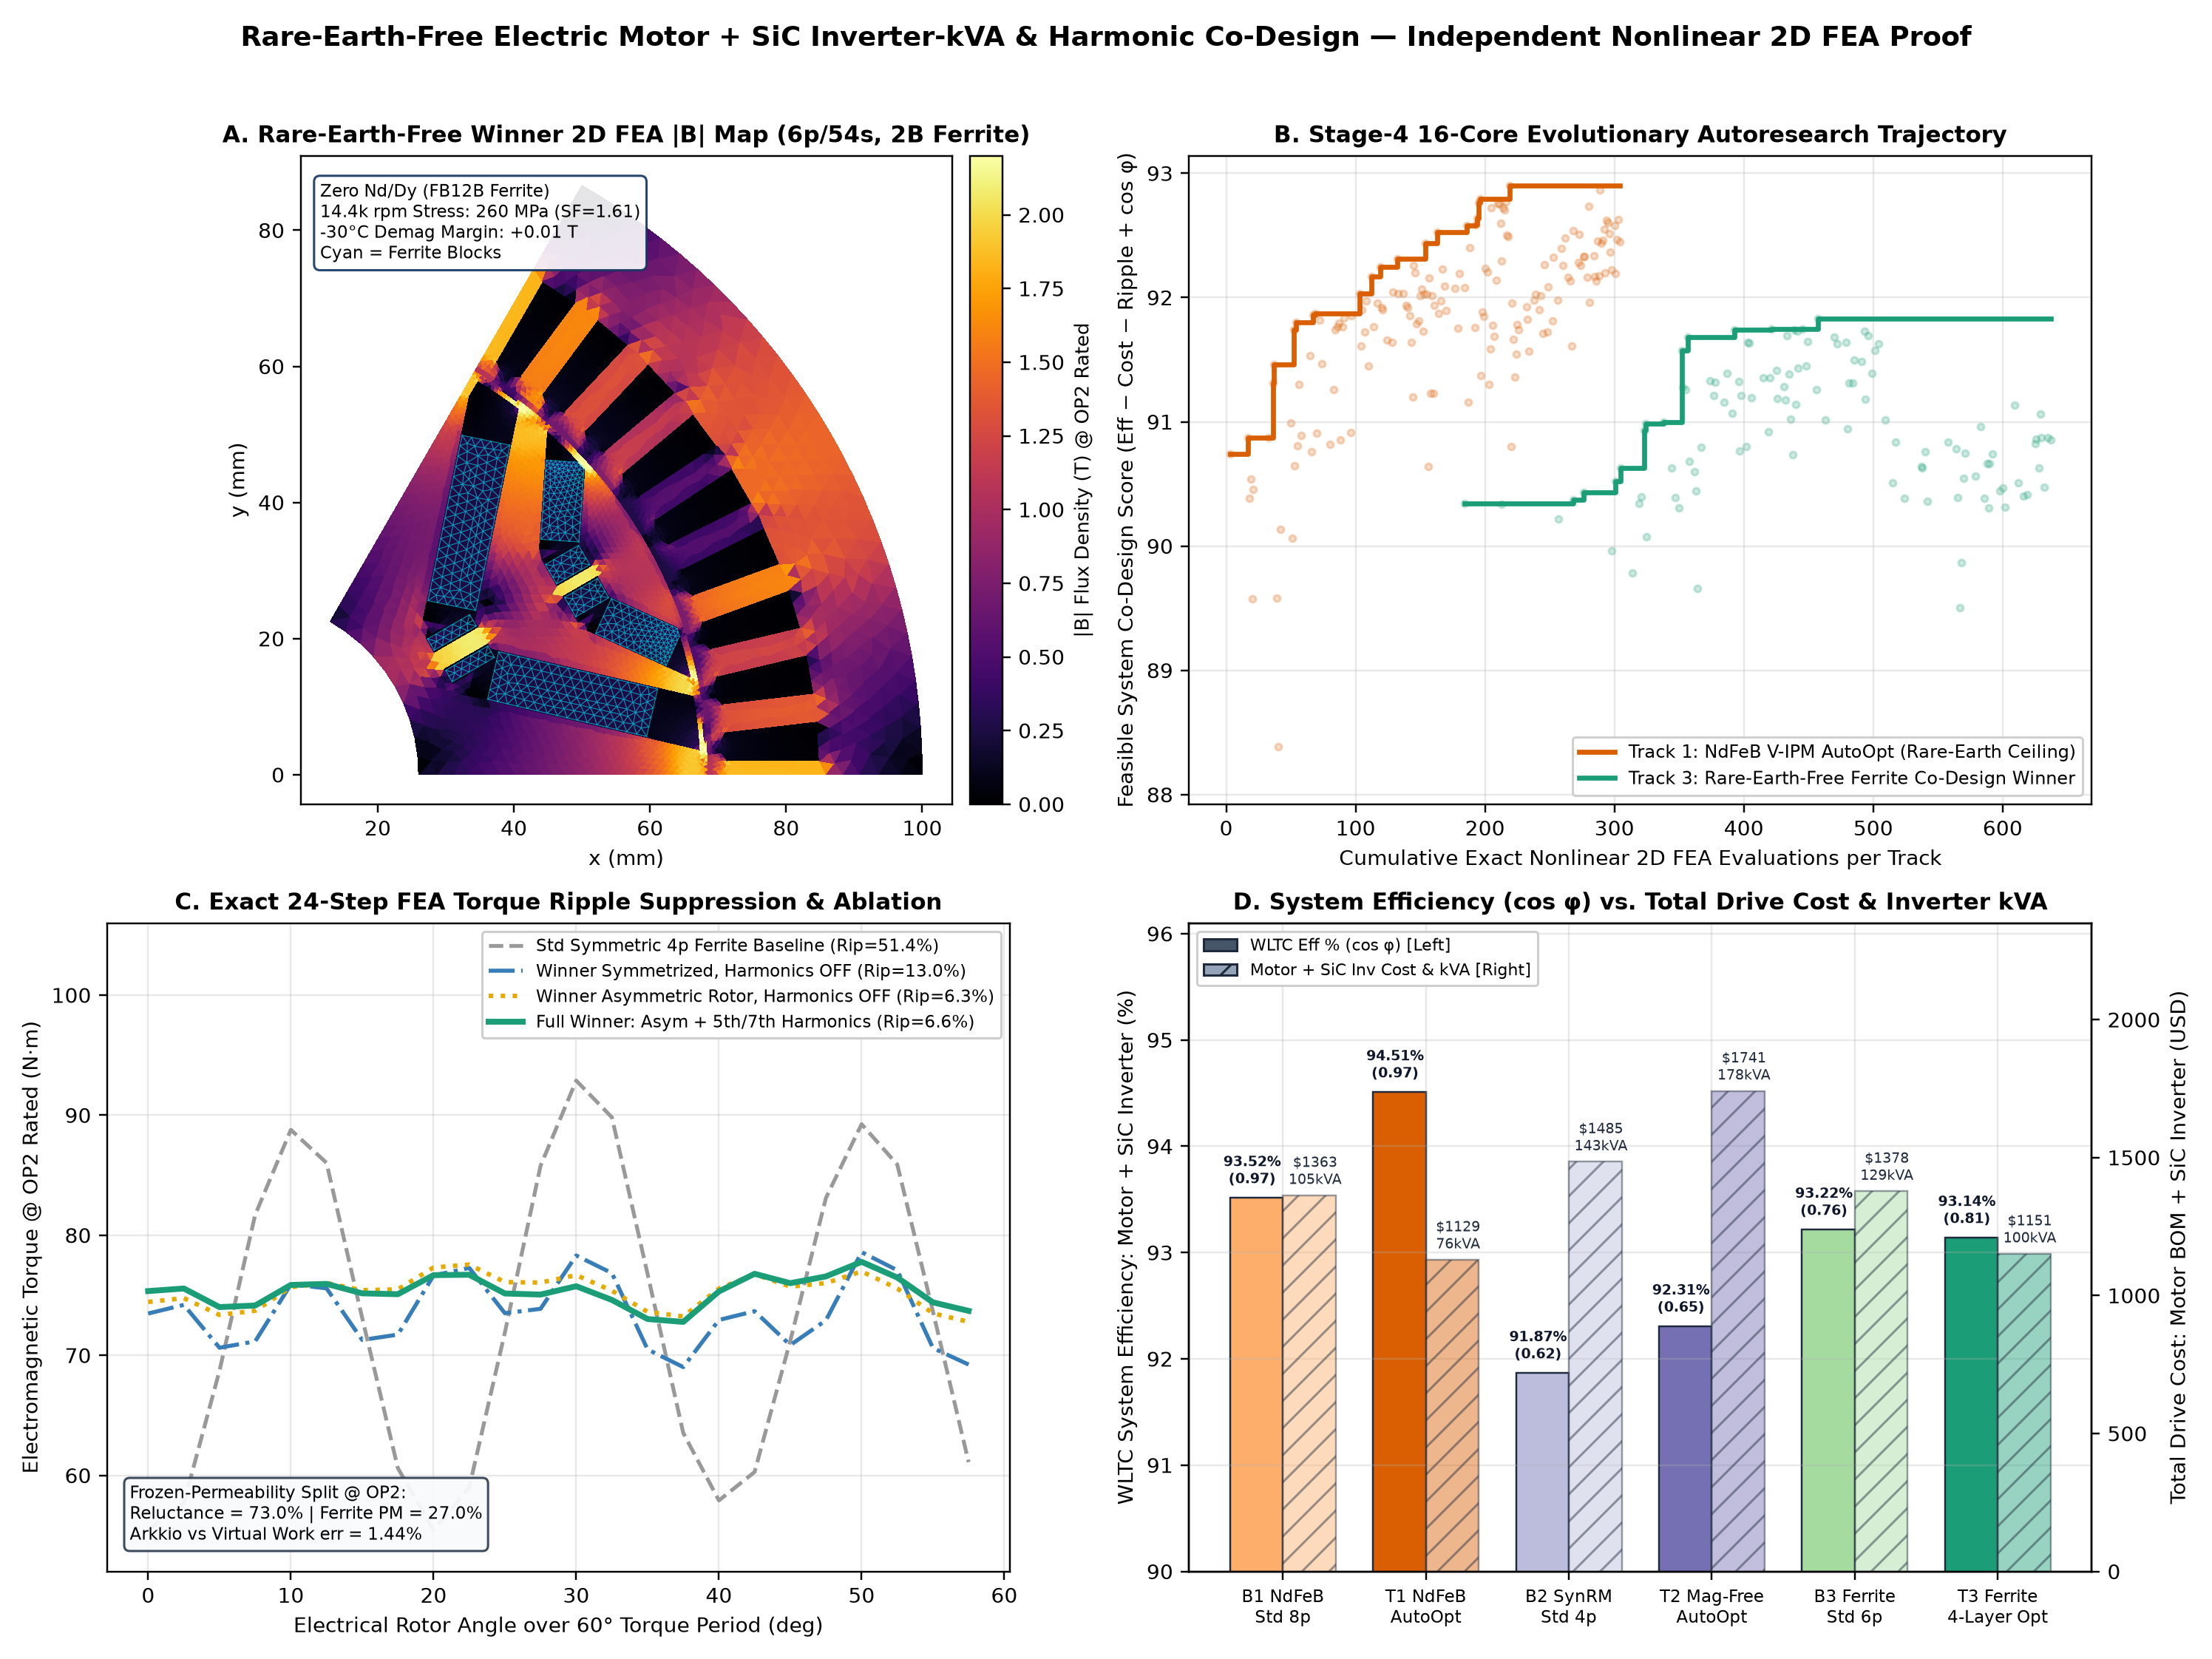
\includegraphics[width=\textwidth]{figures/motor_autoresearch_proof.png}
  \caption{\textbf{Rare-Earth-Free Electric Motor + SiC Inverter-kVA Co-Design Proof ($1{,}296$ Exact Nonlinear 2D FEA Evaluations).} (A) Nonlinear 2D FEA $|B|$ flux-density map of the rare-earth-free winner \texttt{T3} (\texttt{6p/54s 2B} asymmetric thick \texttt{FB12B} ceramic ferrite, cyan mesh) at rated \texttt{OP2}, showing saturated structural posts holding $14{,}400\;\text{rpm}$ load ($\text{SF}=1.61$ at $m=1.0$, $1.52$ at $m=0.65$) and $+0.019\;\text{T}$ $-30\,^\circ\text{C}$ demagnetization margin. (B) Stage-4 16-core evolutionary trajectories for \texttt{T1} (\texttt{NDFEB\_OPT}) and \texttt{T3} (\texttt{FERRITE\_CO\_DESIGN\_OPT}). (C) Exact 24-step torque waveforms at \texttt{OP2} isolating the $-51.5\%$ ripple reduction from rotor asymmetry alone ($13.0\%\to 6.3\%$, vs.\ $51.4\%$ textbook baseline) and exact frozen-permeability split ($73.0\%$ reluctance / $27.0\%$ ferrite PM). (D) WLTC system efficiency ($\cos\phi$) vs.\ total drive cost (motor BOM + SiC inverter kVA).}
  \label{fig:motor_proof}
\end{figure*}

Stage-4 evolution ran $1{,}024$ fast exact FEA evaluations (`mesh=1.25, n_steps=6`) across three tracks followed by a $272$-eval anti-aliased high-resolution polish (`mesh=1.0, n_steps=12`) after detecting 18th-slot-harmonic Nyquist aliasing on \texttt{6p/54s} at $n_{\text{steps}}=6$. Table~\ref{tab:motor_main} and Fig.~\ref{fig:motor_proof} report the complete benchmark verified on a $2\times$ refined mesh (`mesh=0.65`, $n_{\text{steps}}=24$).

\begin{table*}[t]
\centering
\caption{Head-to-Head EV Traction Motor + 400 V SiC Inverter Benchmark (Stage-4 Winners Verified at $2\times$ Fine Mesh \texttt{0.65}, $n_{\text{steps}}=24$).}
\label{tab:motor_main}
\scriptsize
\begin{tabular}{@{}lllrrrrrrrrl@{}}
\toprule
\textbf{ID} & \textbf{Topology} & \textbf{Magnet (kg / BOM)} & \textbf{$\eta_{\text{sys}}$ (\%)} & \textbf{$\cos\phi$} & \textbf{Rip (\%)} & \textbf{$T_{\text{pk}}$} & \textbf{Inv kVA} & \textbf{Sys Cost} & \textbf{SF} & \textbf{Demag} & \textbf{Status} \\
\midrule
\texttt{B1} Std NdFeB & \texttt{8p/48s 2B} & \texttt{N42SH} (1.45 / \$167) & 93.52 & 0.975 & 32.90 & 188.4 & 105.5 & \$1{,}363 & 2.53 & $+$0.250 T & Fail (Rip) \\
\texttt{B2} Std SynRM & \texttt{4p/36s 3B} & None (0.00 / \$0) & 91.87 & 0.622 & 11.60 & 156.6 & 143.4 & \$1{,}485 & 1.34 & N/A & Fail (SF, $T_{\text{pk}}$) \\
\texttt{B3} Std Ferrite & \texttt{6p/36s 3B} & \texttt{FB12B} (1.75 / \$10) & 93.22 & 0.760 & 18.40 & 186.8 & 128.7 & \$1{,}378 & 1.38 & $-$0.084 T & Fail (SF, Dem) \\
\midrule
\texttt{T1} AutoOpt NdFeB & \texttt{6p/54s 2B} & \texttt{N42SH} (1.27 / \$146) & \textbf{94.44} & \textbf{0.972} & 11.08 & \textbf{185.2} & \textbf{75.8} & \textbf{\$1{,}128} & \textbf{1.67} & $+$0.305 T & \textbf{PASS} \\
\texttt{T2} AutoOpt SynRM & \texttt{4p/48s 4B} & None (0.00 / \$0) & 92.31 & 0.652 & 13.65 & 162.1 & 178.5 & \$1{,}747 & 1.52 & N/A & Fail ($T_{\text{pk}}$) \\
\textbf{\texttt{T3} AutoOpt Ferrite} & \textbf{\texttt{6p/54s 2B}} & \textbf{\texttt{FB12B} (2.23 / \$12)} & \textbf{93.10} & \textbf{0.809} & \textbf{9.46} & \textbf{182.3} & \textbf{99.8} & \textbf{\$1{,}153} & \textbf{1.52} & \textbf{$+$0.019 T} & \textbf{PASS} \\
\bottomrule
\end{tabular}
\end{table*}

\subsection{Three Physical Breakthroughs Discovered}
\begin{enumerate}\setlength{\itemsep}{1pt}
  \item \textbf{Reluctance-Dominated Torque + Ferrite Inverter De-Bloating:} Exact frozen-permeability separation \citep{chu2013frozen} at rated \texttt{OP2} proves \texttt{T3} derives $73.0\%$ of its torque ($54.9\;\text{Nm}$) from free rotor saliency and only $27.0\%$ ($20.3\;\text{Nm}$) from ceramic ferrite (vs.\ $51.3\%$ PM / $48.7\%$ Rel for \texttt{T1}). Crucially, that $27\%$ ferrite flux boosts $\cos\phi$ from $0.652$ (\texttt{T2}) to $0.809$ (\texttt{T3}), collapsing the SiC inverter from $178.5\;\text{kVA}$ to $99.8\;\text{kVA}$ ($-\$590$ in SiC hardware) and beating commercial \texttt{8p} NdFeB (\texttt{B1}, $\$1{,}363$, $105.5\;\text{kVA}$) by $-\$210$ ($-15.4\%$).
  \item \textbf{Asymmetric Thick Double-V Architecture Solves Ripple \& Cold-Soak Demagnetization Simultaneously:} Enlarging the rotor OD to $137.05\;\text{mm}$ ($+15.1\;\text{mm}$ over \texttt{T1}) enables two deep $7.44\;\text{mm}$ / $5.84\;\text{mm}$ ferrite barriers that resist $-30\,^\circ\text{C}$ demagnetization ($+0.019\;\text{T}$ margin at $115\%$ launch; $>94\%$ area still reversible even at $150\%$ short-circuit surge) while heavy $2.90\;\text{mm}$ / $1.81\;\text{mm}$ structural posts preserve $\text{SF}\ge 1.52$ at $14{,}400\;\text{rpm}$. Same-hardware 24-step ablation at \texttt{OP2} (Fig.~\ref{fig:motor_proof}C) proves that asymmetric wing skew ($+2.87^\circ$ inner / $+0.51^\circ$ outer) alone slashes torque ripple by $51.5\%$ ($13.0\%\to 6.3\%$), whereas 5th/7th harmonic injection proves unnecessary once geometric asymmetry is optimized ($6.6\%$).
  \item \textbf{Exact SiC / Rare-Earth Cost Crossover Law:} Compared to autoresearch-optimized Dy-NdFeB (\texttt{T1}, $\$1{,}128$), \texttt{T3} saves $\$134$ in magnet BOM while needing $+24.0\;\text{kVA}$ more SiC inverter capacity, putting \texttt{T3} within $\$25$ ($+2.2\%$) today and making rare-earth-free ferrite \emph{strictly cheaper than optimized Dy-NdFeB} whenever SiC falls below $\$6.46/\text{kVA}$ or Dy-NdFeB rises above $\$135/\text{kg}$.
\end{enumerate}

\section{Independent 5-Test FEA Verification Audit}

Table~\ref{tab:motor_verif} summarizes all five independent adversarial checks: (1) $2\times$ mesh & $4\times$ time-step convergence (`mesh=1.25/n6 -> 0.65/n24`, $|\Delta\eta_{\text{sys}}|\le 0.19\;\text{pt}$); (2) Arkkio vs.\ magnetic co-energy Virtual Work ($\partial W'/\partial\theta$) agreement within $0.04\%\text{--}1.44\%$; (3) $0.00\%$ frozen-permeability linear superposition error; (4) worst-case $115\%/135\%/150\%$ peak surge demagnetization audit; and (5) 32-draw correlated manufacturing tolerance Monte Carlo ($\pm 0.08\;\text{mm}$ stamping rib/bridge, $\pm 0.04\;\text{mm}$ air gap) confirming $30/32$ ($93.8\%$) full feasibility and $\min\text{SF}=1.58$ for \texttt{T3}.

\begin{table}[h]
\centering
\caption{Five-Test Independent Verification Summary for Stage-4 Winners.}
\label{tab:motor_verif}
\scriptsize
\begin{tabular}{@{}lrrr@{}}
\toprule
\textbf{Verification Metric} & \textbf{\texttt{T1} NdFeB} & \textbf{\texttt{T2} SynRM} & \textbf{\texttt{T3} Ferrite} \\
\midrule
Mesh/Step Drift $\Delta\eta_{\text{sys}}$ & $0.00\;\text{pt}$ & $-0.13\;\text{pt}$ & $-0.19\;\text{pt}$ \\
Arkkio vs.\ Virtual Work Error & $0.87\%$ & $0.04\%$ & $1.44\%$ \\
Frozen-Perm.\ PM / Rel Split & $51.3 / 48.7\%$ & $0 / 100\%$ & $27.0 / 73.0\%$ \\
Frozen-Perm.\ Superpos.\ Error & $0.00\%$ & $0.00\%$ & $0.00\%$ \\
150\% Surge Area $< B_{\text{knee}}$ & $0.00\%$ & N/A & $5.84\%$ \\
32-Draw MC $\eta_{\text{sys}}$ (\%) & $94.46\pm 0.04$ & $92.49\pm 0.07$ & $93.23\pm 0.10$ \\
32-Draw MC Cost (USD) & $\$1{,}130\pm 4$ & $\$1{,}742\pm 5$ & $\$1{,}150\pm 5$ \\
32-Draw MC Feas / Min SF & $32/32$ (2.04) & $0/32$ (1.43) & $30/32$ (1.58) \\
\bottomrule
\end{tabular}
\end{table}

\appendix
\section{Manufacturable CAD & Control Specs (\texttt{T3})}

Table~\ref{tab:cad_motor} lists the exact stator, rotor, and 5-point $(I_d, I_q)$ schedule exported from \texttt{motor\_engineering\_specs.json} for immediate wire-EDM / laser lamination prototyping. Three 3D physical effects---axial rotor skew, end-region 3D flux fringing, and transient thermal cooling jacket gradients---define the next dynamometer validation step.

\begin{table}[h]
\centering
\caption{Rare-Earth-Free Winner \texttt{T3} (\texttt{6p/54s 2B}) CAD \& WLTC Schedule.}
\label{tab:cad_motor}
\scriptsize
\begin{tabular}{@{}lr|lr@{}}
\toprule
\textbf{Stator / Envelope} & \textbf{Value} & \textbf{Asym.\ 2B Rotor} & \textbf{B1 / B2} \\
\midrule
Stator OD $\times$ Stack & $200\times 140\;\text{mm}$ & Center $u$ (mm) & $37.20$ / $56.91$ \\
Rotor OD / Shaft OD & $137.05$ / $52\;\text{mm}$ & Thickness (mm) & $7.44$ / $5.84$ \\
Air Gap / Yoke & $0.685$ / $15.15\;\text{mm}$ & Wing L/R ($^\circ$) & $24.1/27.0$ ; $15.9/16.5$ \\
Tooth $k_t$ / Slot Open & $0.499$ / $1.84\;\text{mm}$ & Bridge / Rib (mm) & $1.17/2.90$ ; $1.06/1.81$ \\
Eff.\ Turns $N_c$ / $R_{\text{ph}}$ & $3.25$ / $43.1\;\text{m}\Omega$ & Mag Fill C/W & $0.88/0.86$ ; $0.80/0.86$ \\
Active Steel/Cu/Fer & $22.0 / 4.3 / 2.2\;\text{kg}$ & Surface Notch & $0.38\;\text{mm}$ @ $24.7^\circ$ \\
\midrule
\multicolumn{4}{@{}l}{\textbf{WLTC $(I_d, I_q, V_{\text{pk}}, \eta_{\text{sys}})$:} \texttt{OP1} $(-62,62\;\text{A}, 87\;\text{V}, 91.4\%)$; \texttt{OP2} $(-105,92\;\text{A}, 211\;\text{V}, 93.4\%)$;} \\
\multicolumn{4}{@{}l}{\texttt{OP3} $(-130,40\;\text{A}, 210\;\text{V}, 94.0\%)$; \texttt{OP4} $(-153,23\;\text{A}, 214\;\text{V}, 92.2\%)$; \texttt{OP5} $(-253,167\;\text{A}, 182.4\;\text{Nm})$.} \\
\bottomrule
\end{tabular}
\end{table}

\section*{AI-Assisted Methodology Disclosure}
This computational study was directed, reviewed, and published by the author using an autonomous multi-agent scientific research pipeline to synthesize literature, draft finite-element code, execute parallel evolutionary evaluations, and run independent verification audits. All governing physics equations, material parameters, finite-element meshes, convergence proofs, and raw data ledgers are openly archived for full independent reproduction.

\bibliographystyle{unsrtnat}
\bibliography{references}

\end{document}
